\chapter{Réalisation du Sprint 2 : Gestion des produits et du stock}

\section{Introduction}

Ce deuxième sprint est consacré à la gestion des produits et du stock. Il permet de mettre en place les fonctionnalités liées à la gestion du catalogue, des catégories, des marques, des fournisseurs et du stock.

Il couvre également les fonctionnalités de panier, de commandes, de facturation et de paiement, afin d'assurer la continuité entre la gestion des produits et les opérations de vente.

\section{Analyse du Sprint}

\subsection{Sprint Backlog}

Le Sprint Backlog regroupe les principales fonctionnalités à réaliser au cours de ce sprint. Il permet de définir les besoins fonctionnels liés à la gestion des produits, du stock, des fournisseurs ainsi qu'aux opérations de commande et de paiement.

\begin{longtable}{|c|>{\RaggedRight\arraybackslash}p{5cm}|>{\RaggedRight\arraybackslash}p{5cm}|c|}
\hline
\textbf{ID} & \textbf{User Story} & \textbf{Critère d'acceptation} & \textbf{Priorité}\\
\hline
\endfirsthead

\hline
\textbf{ID} & \textbf{User Story} & \textbf{Critère d'acceptation} & \textbf{Priorité}\\
\hline
\endhead


US1 &
En tant qu'employé, je souhaite consulter la liste des produits afin de visualiser les produits disponibles. &
La liste des produits est affichée avec leurs principales informations. &
Haute
\\
\hline


US2 &
En tant qu'employé, je souhaite rechercher, filtrer et trier les produits afin de retrouver rapidement un produit. &
Les produits peuvent être recherchés, filtrés et triés selon les critères disponibles. &
Haute
\\
\hline


US3 &
En tant qu'employé, je souhaite ajouter, modifier et supprimer un produit afin de maintenir le catalogue à jour. &
Un produit peut être créé, modifié ou supprimé avec succès. &
Haute
\\
\hline


US4 &
En tant qu'employé, je souhaite gérer les catégories et les marques afin d'organiser les produits. &
Les catégories et les marques peuvent être ajoutées, modifiées ou supprimées selon les fonctionnalités disponibles. &
Haute
\\
\hline


US5 &
En tant qu'employé, je souhaite consulter et gérer le stock afin de suivre les quantités disponibles. &
Les quantités et les informations du stock peuvent être consultées et mises à jour. &
Haute
\\
\hline


US6 &
En tant qu'employé, je souhaite enregistrer une réception de livraison afin de mettre à jour le stock. &
La réception augmente la quantité disponible et enregistre le mouvement correspondant. &
Haute
\\
\hline


US7 &
En tant qu'employé, je souhaite consulter les mouvements de stock afin de suivre les entrées et les sorties. &
Les mouvements sont affichés avec leurs informations principales et leur date. &
Moyenne
\\
\hline


US8 &
En tant qu'employé, je souhaite identifier les produits en stock faible afin d'anticiper leur réapprovisionnement. &
Les produits dont la quantité est inférieure ou égale au seuil sont identifiés. &
Haute
\\
\hline


US9 &
En tant qu'employé, je souhaite gérer les fournisseurs afin de maintenir les informations d'approvisionnement à jour. &
Un fournisseur peut être consulté, ajouté, modifié ou supprimé. &
Moyenne
\\
\hline


US10 &
En tant que client, je souhaite gérer mon panier afin de préparer ma commande. &
Les produits peuvent être ajoutés, modifiés, supprimés ou retirés du panier et le total est calculé. &
Haute
\\
\hline


US11 &
En tant que client, je souhaite créer une commande et consulter sa facture afin de suivre mon achat. &
La commande est enregistrée et les informations de facturation sont disponibles. &
Haute
\\
\hline


US12 &
En tant que client, je souhaite effectuer un paiement afin de confirmer ma commande. &
Le paiement est enregistré, la commande est confirmée et le stock est mis à jour. &
Haute
\\
\hline


\caption{Sprint Backlog du Sprint 2}
\label{tab:sprint2-backlog}

\end{longtable}

\section{Conception}

\subsection{Diagramme de Cas d'Utilisation}

Le diagramme de cas d'utilisation du Sprint 2 présente les interactions entre les différents acteurs du système et les principales fonctionnalités développées pour la gestion des produits, du stock, des fournisseurs ainsi que pour les opérations commerciales liées au panier, aux commandes et au paiement.

Dans ce sprint, quatre acteurs sont considérés : User, Customer, Employee et Admin. L'acteur User représente l'utilisateur générique du système, tandis que Customer, Employee et Admin correspondent à ses spécialisations. Cette généralisation permet de représenter la hiérarchie des acteurs tout en distinguant les fonctionnalités accessibles selon leur rôle.

Le Customer intervient principalement dans la consultation des produits, la gestion de son panier et les opérations relatives à ses propres commandes. L'Employee intervient dans les opérations de gestion qui lui sont accessibles selon les permissions qui lui sont attribuées. L'Admin dispose de droits étendus sur les fonctionnalités de gestion.

Les permissions d'accès ne sont pas représentées comme des acteurs distincts. Elles constituent des mécanismes de contrôle d'accès permettant de déterminer les fonctionnalités accessibles à un employé.

\subsubsection{Description des acteurs}

\begin{itemize}
\item \textbf{User :} représente l'acteur générique dont héritent les différents types d'utilisateurs de l'application. Il permet de représenter la généralisation commune aux acteurs Customer, Employee et Admin.
\item \textbf{Customer :} il peut consulter les produits, gérer son panier, confirmer une commande, consulter ses commandes et annuler une commande selon les règles métier de l'application.
\item \textbf{Employee :} il accède aux fonctionnalités de gestion selon les permissions qui lui sont attribuées. Il peut notamment intervenir dans la gestion des produits, des catégories, des marques, du stock, des fournisseurs et des commandes lorsque les autorisations correspondantes lui sont accordées.
\item \textbf{Admin :} il dispose de droits étendus sur les fonctionnalités de gestion. Il peut notamment gérer les produits, les catégories, les marques, le stock, les fournisseurs et les commandes.
\end{itemize}

\subsubsection{Principaux cas d'utilisation}

Les principaux cas d'utilisation du Sprint 2 sont regroupés selon les domaines fonctionnels suivants :

\begin{itemize}
\item \textbf{Gestion du catalogue :} consulter les produits, gérer les produits, gérer les catégories et gérer les marques. La consultation du catalogue comprend également la recherche, le filtrage, le tri et la pagination.
\item \textbf{Gestion du stock :} consulter le stock, réceptionner une livraison et consulter les mouvements de stock.
\item \textbf{Gestion des fournisseurs :} consulter, rechercher, ajouter, modifier et supprimer un fournisseur.
\item \textbf{Gestion du panier :} consulter le panier, ajouter des produits, modifier les quantités, supprimer des articles et vider le panier.
\item \textbf{Gestion des commandes :} confirmer une commande, consulter ses commandes, annuler une commande, consulter les commandes et modifier leur statut.
\item \textbf{Paiement :} effectuer un paiement associé à une facture.
\end{itemize}

\subsubsection{Diagramme de Cas d'Utilisation du Sprint 2}

La figure suivante présente le diagramme de cas d'utilisation correspondant aux principales fonctionnalités développées au cours du Sprint 2.

\begin{figure}[H]
\centering
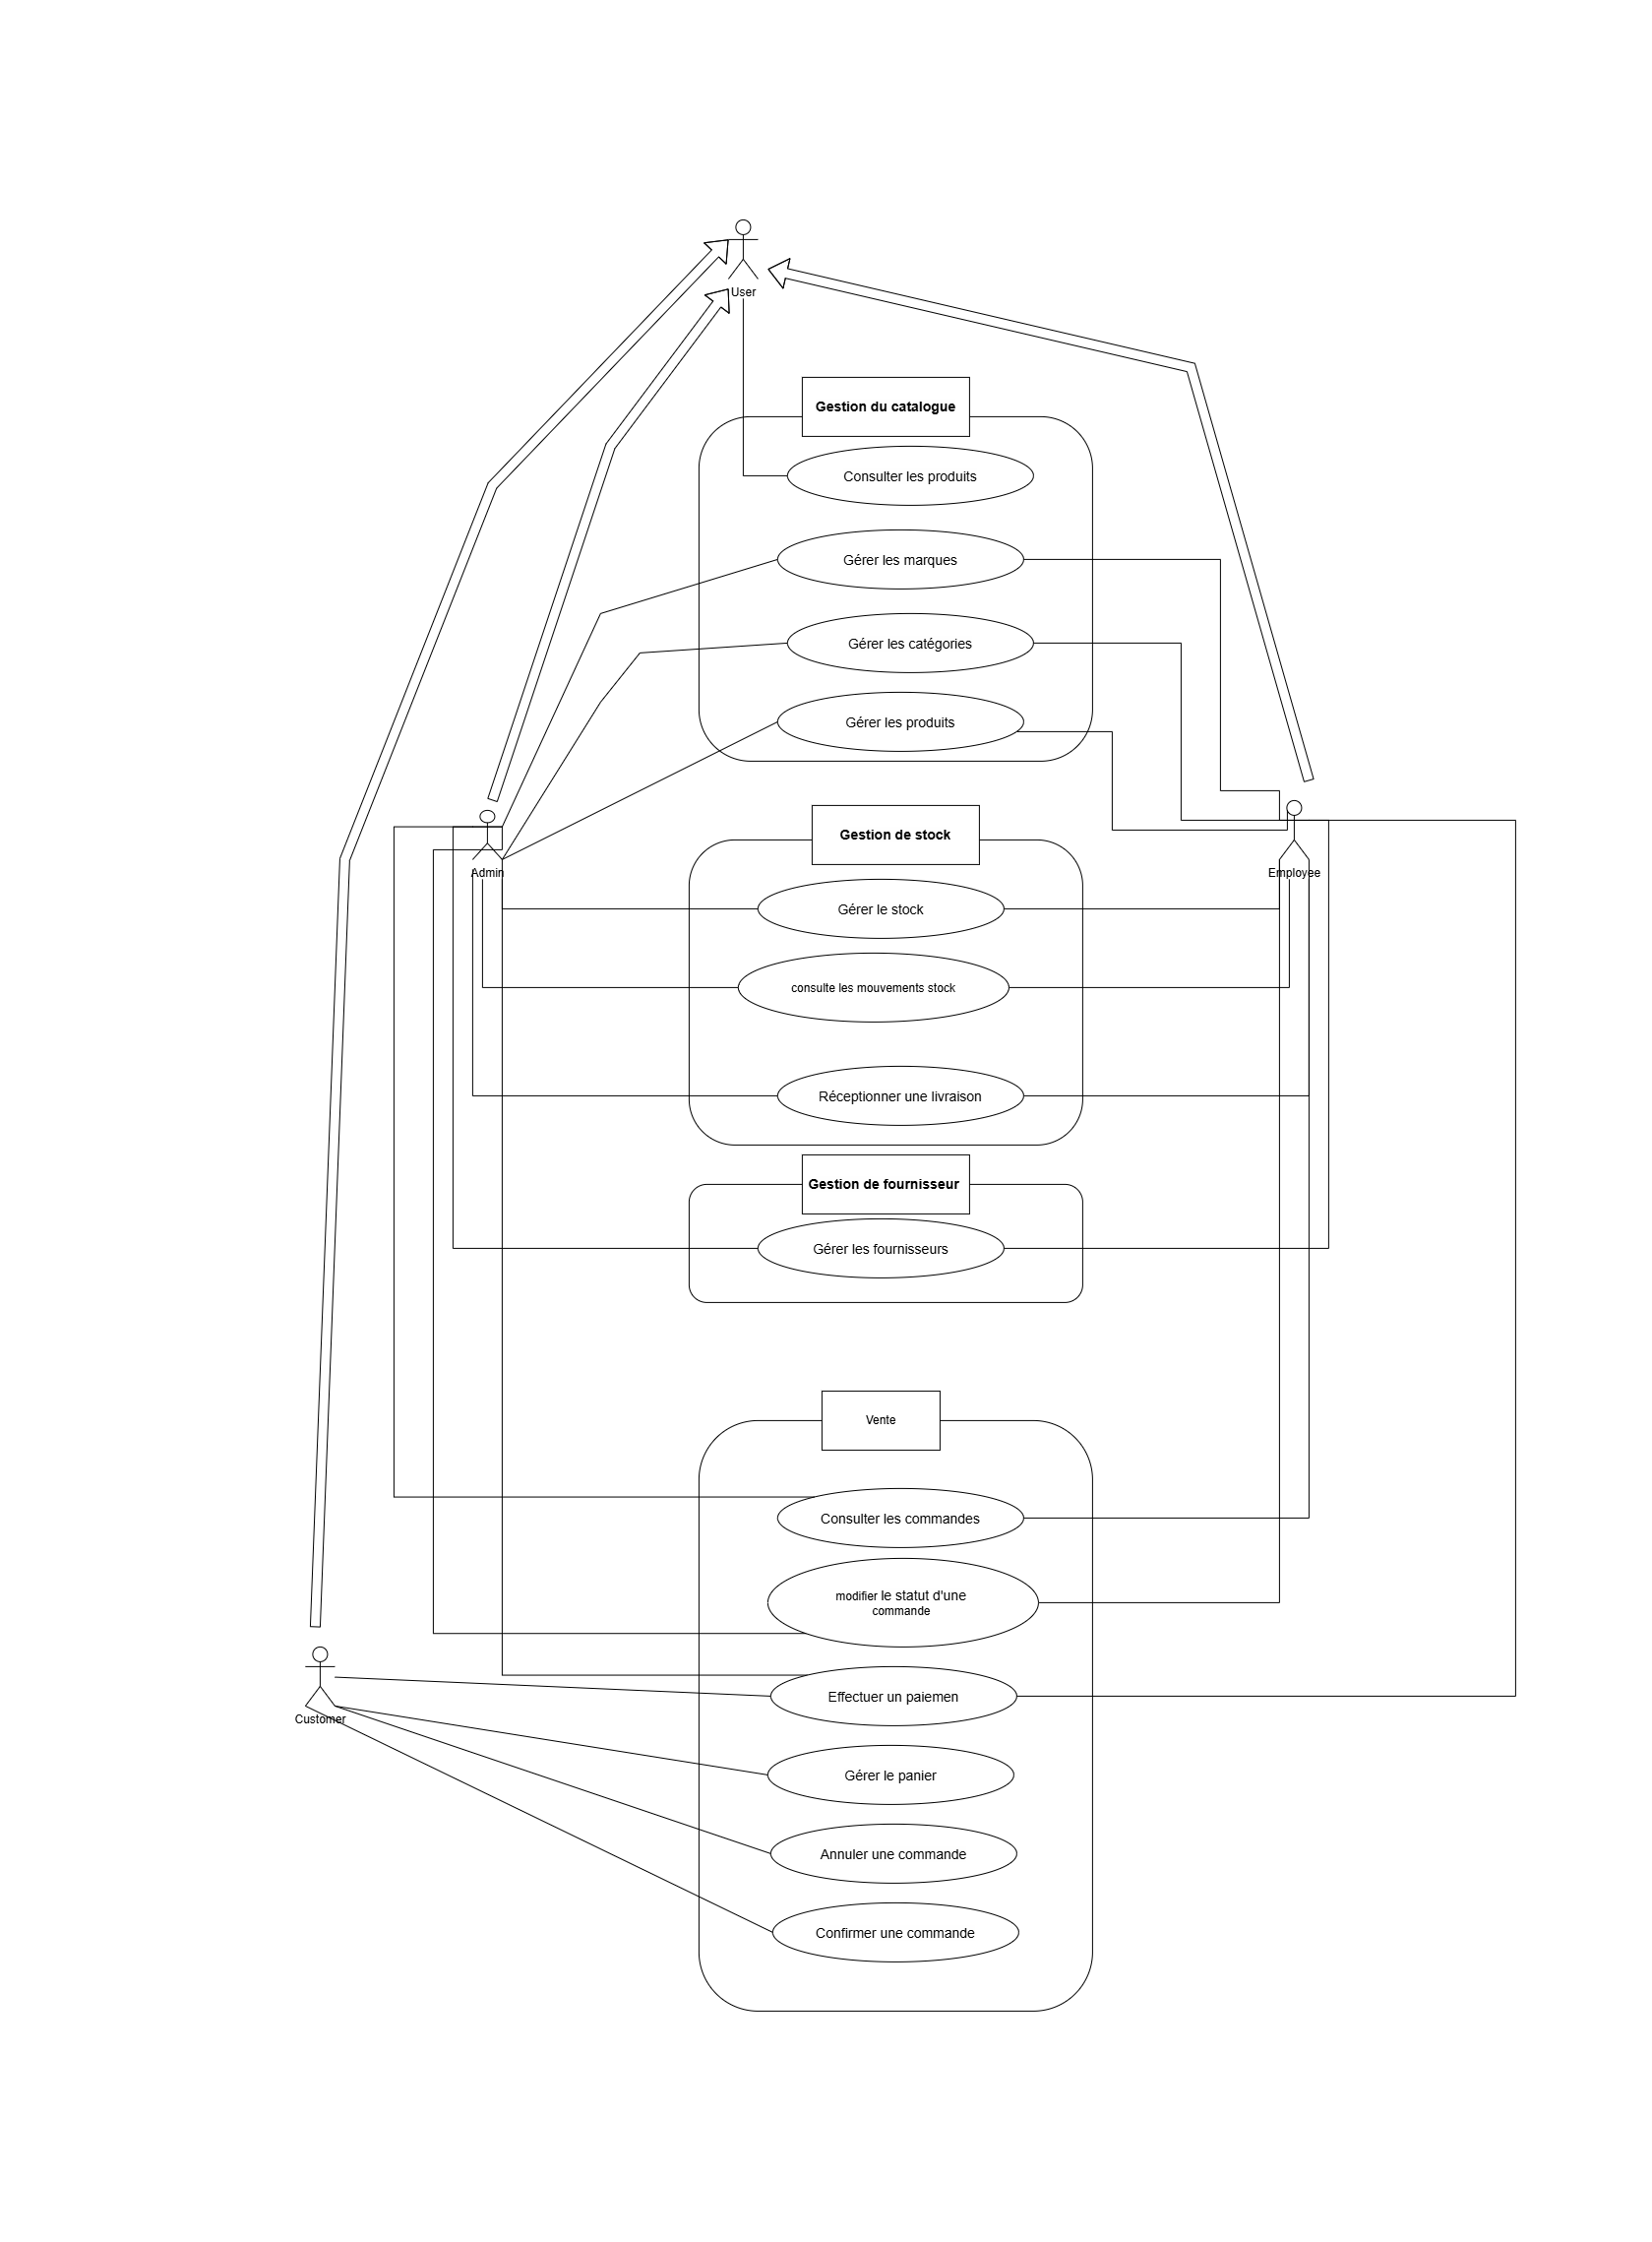
\includegraphics[width=\textwidth]{images/uml/sprint2_GestionProduct.png}
\caption{Diagramme de cas d'utilisation du Sprint 2}
\label{fig:sprint2-use-case}
\end{figure}

\subsubsection{Description des Cas d'Utilisation Principaux}

\paragraph{UC1 : Consulter les produits}
Ce cas d'utilisation permet aux utilisateurs de consulter les produits disponibles dans le catalogue. La consultation peut être réalisée avec différents paramètres permettant d'organiser les résultats affichés.

\paragraph{UC2 : Gérer les produits}
Ce cas d'utilisation permet aux utilisateurs disposant des autorisations nécessaires d'ajouter, de modifier et de supprimer les produits du catalogue.

\paragraph{UC3 : Gérer les catégories}
Ce cas d'utilisation permet de consulter et d'ajouter les catégories utilisées pour organiser les produits du catalogue.

\paragraph{UC4 : Gérer les marques}
Ce cas d'utilisation permet de consulter, d'ajouter et de supprimer les marques associées aux produits.

\paragraph{UC5 : Gérer le stock}
Ce cas d'utilisation permet de consulter et de suivre les informations relatives aux quantités disponibles pour les différents produits.

\paragraph{UC6 : Réceptionner une livraison}
Ce cas d'utilisation permet d'enregistrer la réception d'une livraison provenant d'un fournisseur. Cette opération entraîne la mise à jour du stock et l'enregistrement du mouvement correspondant.

\paragraph{UC7 : Consulter les mouvements de stock}
Ce cas d'utilisation permet de consulter les mouvements enregistrés afin de suivre les opérations ayant affecté le stock.

\paragraph{UC8 : Gérer les fournisseurs}
Ce cas d'utilisation permet de consulter, rechercher, ajouter, modifier et supprimer les informations relatives aux fournisseurs.

\paragraph{UC9 : Gérer le panier}
Ce cas d'utilisation permet au client de consulter son panier, d'ajouter des produits, de modifier leurs quantités, de supprimer des articles ou de vider le panier.

\paragraph{UC10 : Confirmer une commande}
Ce cas d'utilisation permet au client de confirmer une commande à partir des produits présents dans son panier. La commande est alors enregistrée dans le système.

\paragraph{UC11 : Consulter ses commandes}
Ce cas d'utilisation permet au client de consulter les commandes qui lui sont associées et de suivre leur état.

\paragraph{UC12 : Annuler une commande}
Ce cas d'utilisation permet au client d'annuler une commande qui lui appartient, sous réserve des règles métier appliquées par l'application.

\paragraph{UC13 : Consulter les commandes}
Ce cas d'utilisation permet aux utilisateurs disposant des autorisations nécessaires de consulter les commandes enregistrées dans le système.

\paragraph{UC14 : Modifier le statut d'une commande}
Ce cas d'utilisation permet aux utilisateurs autorisés de modifier le statut d'une commande afin d'assurer son suivi au cours du processus de traitement.

\paragraph{UC15 : Effectuer un paiement}
Ce cas d'utilisation permet d'enregistrer le paiement associé à une facture selon les autorisations définies dans l'application.

\subsection{Diagramme de Séquence}

Afin d'illustrer le fonctionnement dynamique des principales fonctionnalités du Sprint 2, trois diagrammes de séquence ont été retenus. Une attention particulière est portée à la gestion du stock, qui constitue le cœur fonctionnel de ce sprint, à travers un diagramme détaillé illustrant la réception d'une livraison et la mise à jour automatique des quantités disponibles.

\subsubsection{Réception d'une livraison et mise à jour du stock}

Ce diagramme illustre le processus central de la gestion du stock : l'enregistrement d'une réception de livraison en provenance d'un fournisseur, la mise à jour du prix d'achat référence chez ce fournisseur, ainsi que la mise à jour automatique de la quantité disponible, du prix moyen pondéré et du mouvement de stock associé.

Le scénario principal est le suivant :

\begin{itemize}
    \item L'employé saisit le produit, le fournisseur, la quantité, le prix unitaire et une note, puis valide la réception.
    \item Le contrôleur transmet la requête au service de gestion des approvisionnements.
    \item Le service vérifie l'existence du produit et du fournisseur.
    \item La référence fournisseur du produit (prix d'achat, date de dernière livraison) est créée ou mise à jour.
    \item Le stock du produit est récupéré, ou créé s'il n'existe pas encore.
    \item Le prix moyen pondéré et la nouvelle quantité disponible sont calculés puis enregistrés.
    \item Si la quantité disponible devient positive, le statut du produit est mis à jour à « En stock ».
    \item Un mouvement de stock de type entrée est enregistré avec le fournisseur, la quantité et le prix unitaire.
    \item Les informations mises à jour du stock sont retournées à l'employé.
\end{itemize}

\begin{figure}[H]
    \centering
    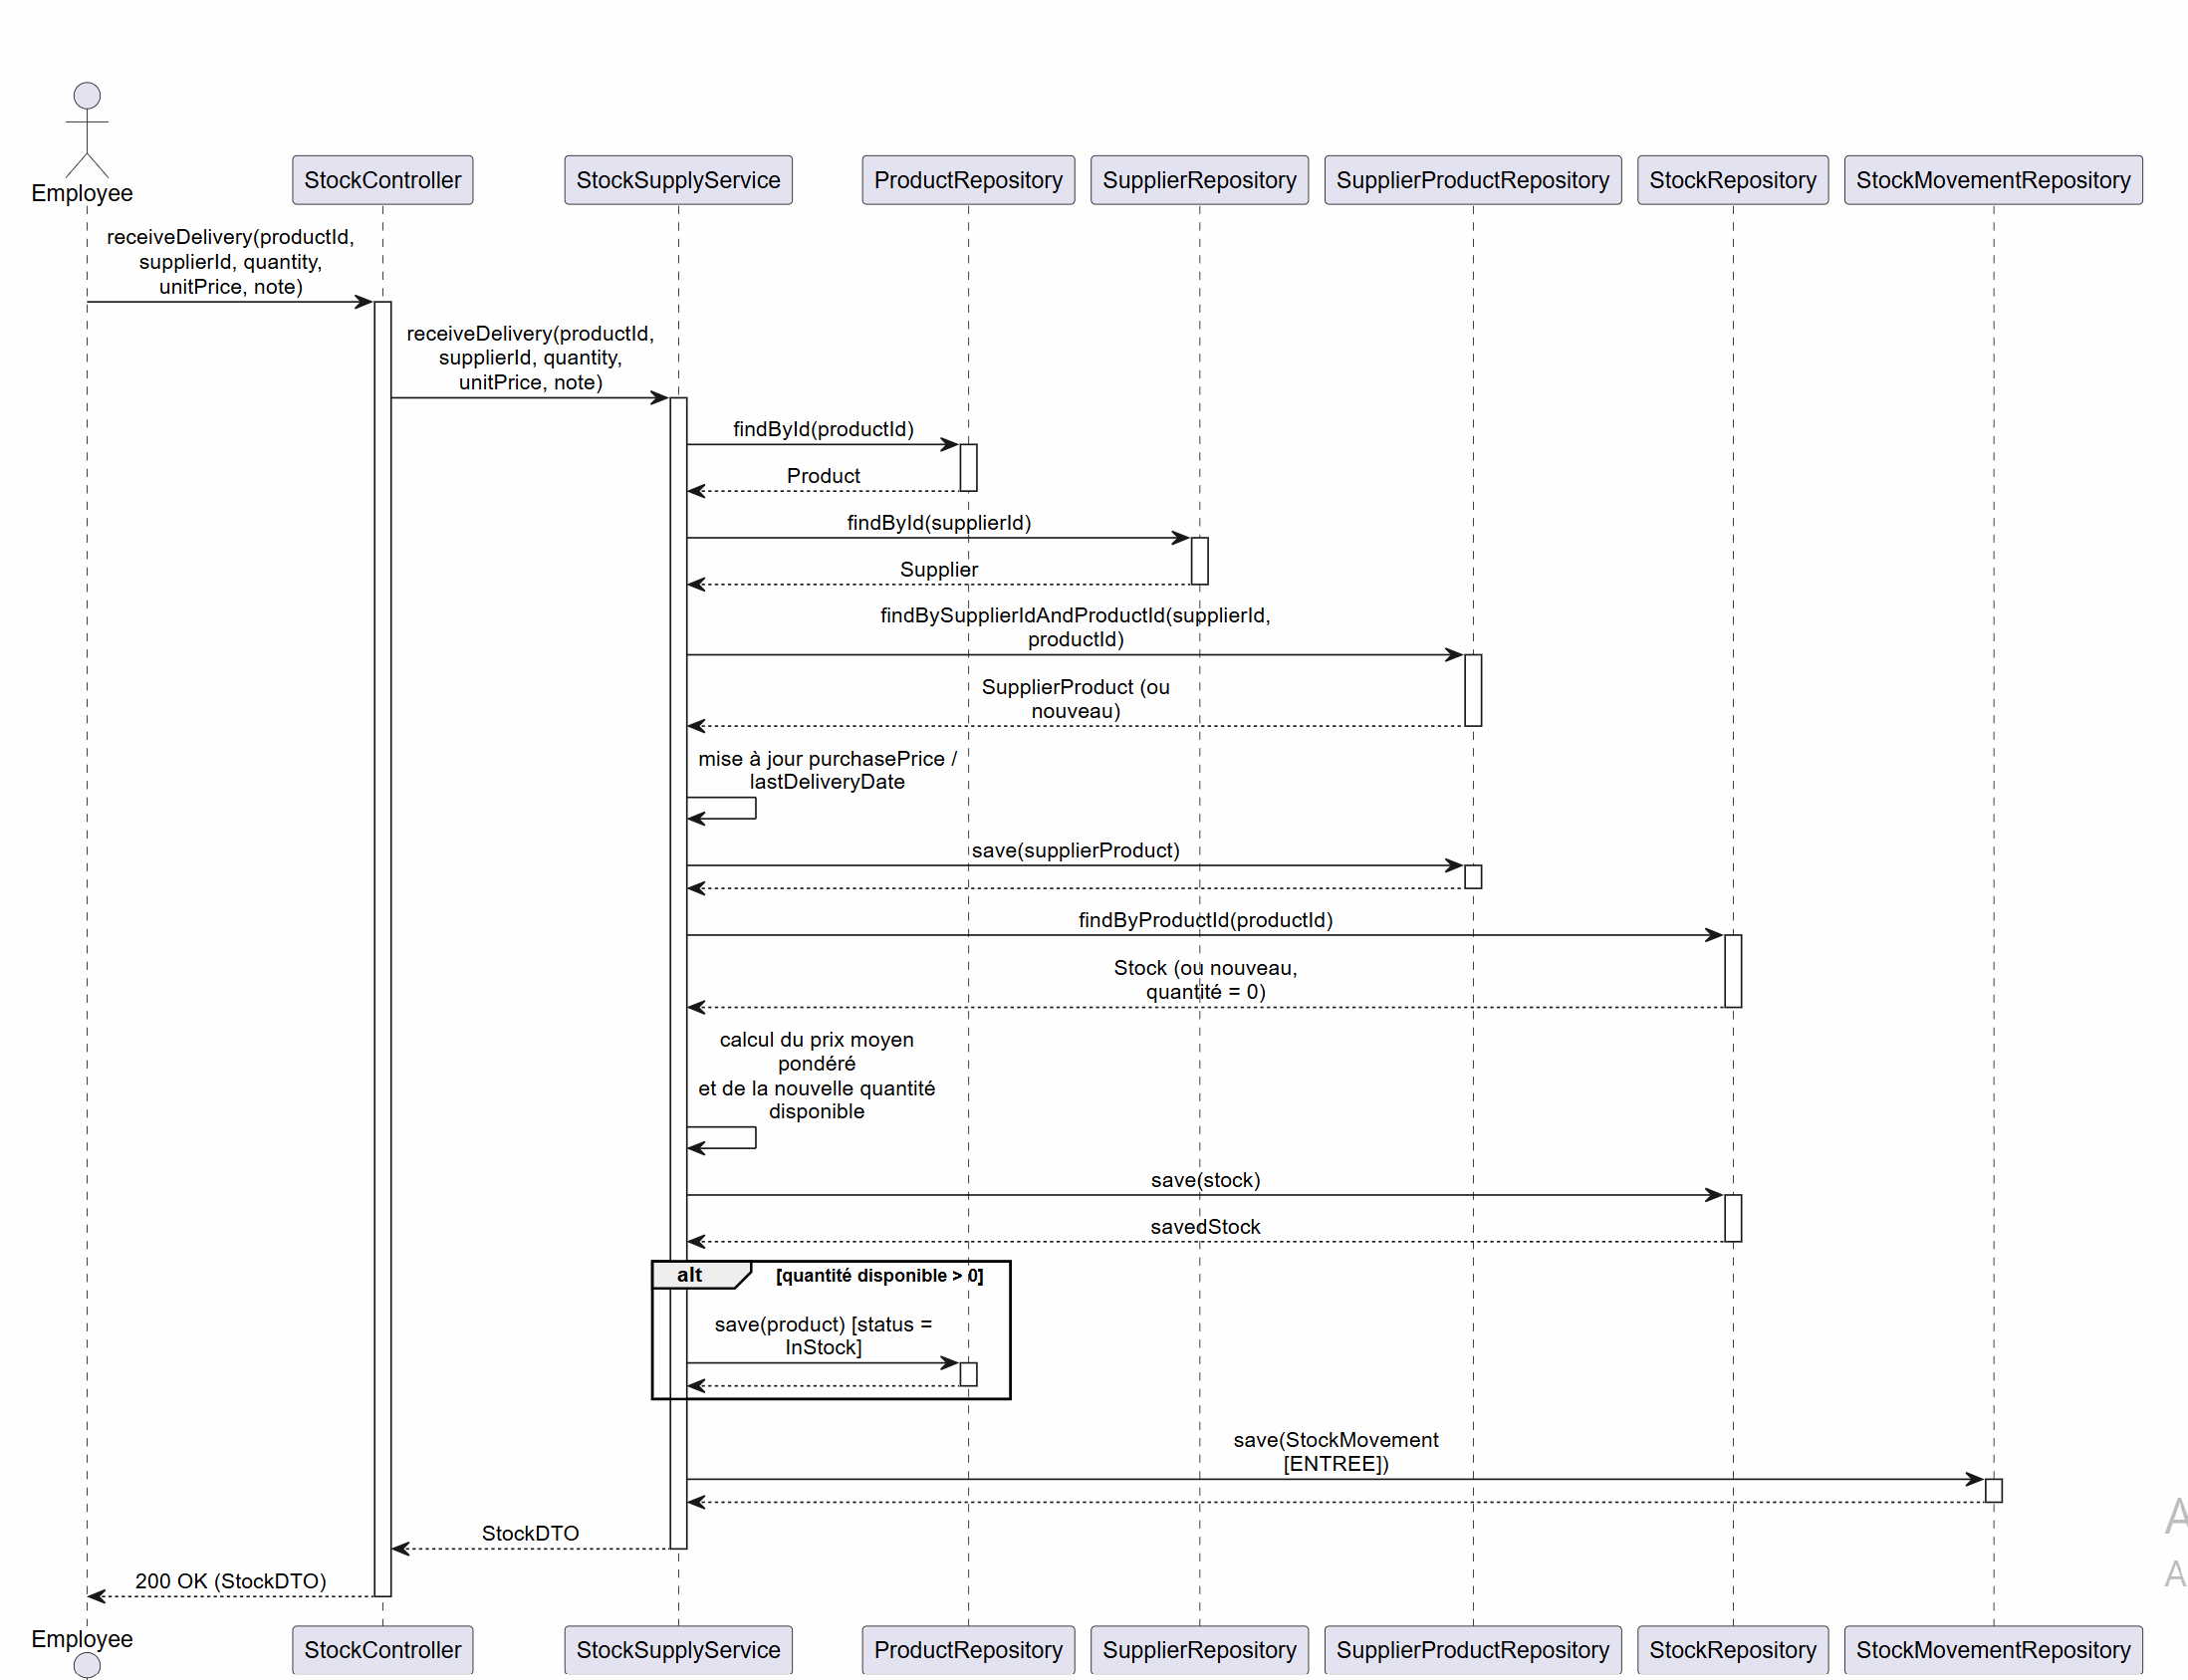
\includegraphics[width=1\textwidth]{images/uml/stockReception.png}
    \caption{Diagramme de séquence - Réception d'une livraison et mise à jour du stock}
    \label{fig:sequence_reception_stock}
\end{figure}

\subsubsection{Ajustement manuel du stock}

Ce diagramme illustre le processus permettant à un employé d'ajuster manuellement la quantité disponible d'un produit, par exemple à la suite d'un inventaire ou d'une correction. Chaque ajustement est automatiquement tracé sous la forme d'un mouvement de stock.

Le scénario principal est le suivant :

\begin{itemize}
    \item L'employé sélectionne un stock et saisit une quantité d'ajustement ainsi qu'un motif.
    \item Le contrôleur transmet la demande au service de gestion du stock.
    \item Le service récupère le stock concerné et calcule la nouvelle quantité disponible.
    \item Si la nouvelle quantité est négative, une erreur est retournée et l'ajustement est rejeté.
    \item Sinon, la quantité disponible et la date de mise à jour du stock sont enregistrées.
    \item Un mouvement de stock est créé, de type entrée si l'ajustement est positif ou de type sortie s'il est négatif.
    \item La confirmation de l'ajustement est retournée à l'employé.
\end{itemize}

\begin{figure}[H]
    \centering
    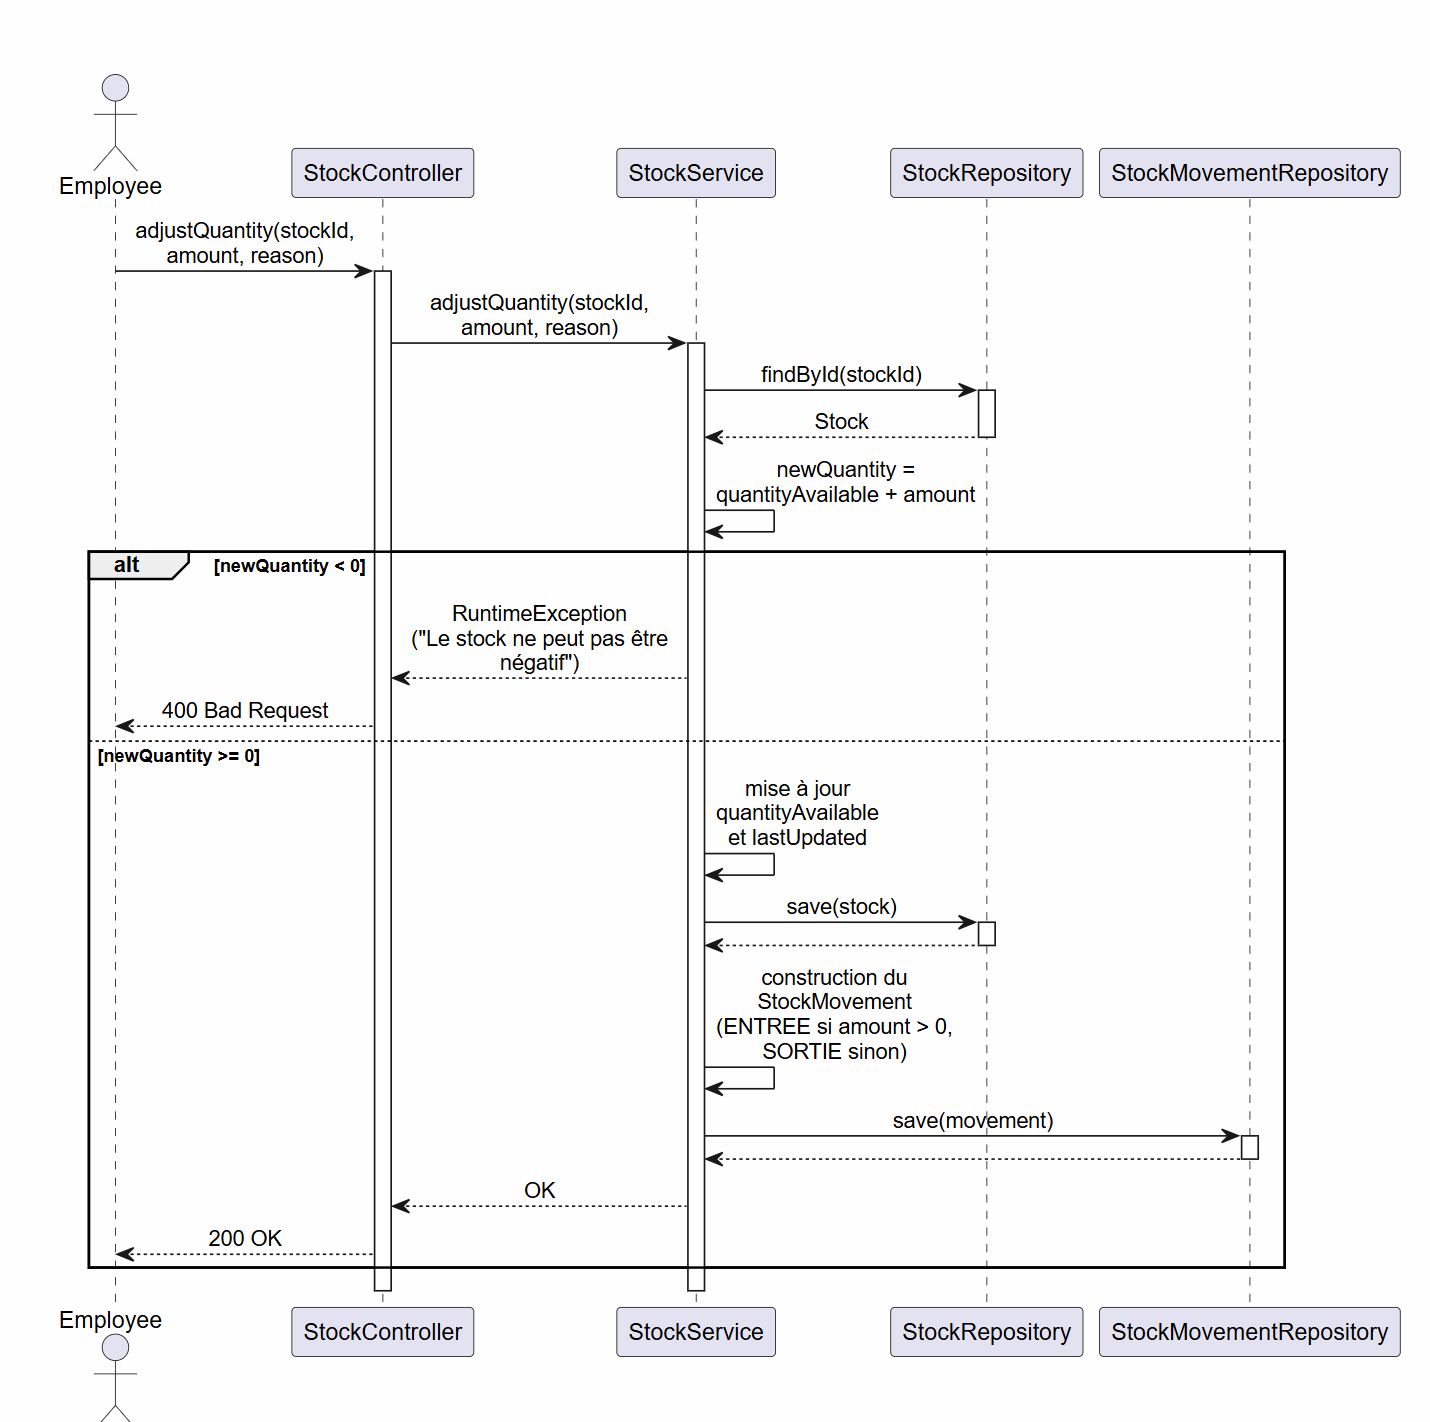
\includegraphics[width=1\textwidth]{images/uml/AjustementStock.png}
    \caption{Diagramme de séquence - Ajustement manuel du stock}
    \label{fig:sequence_ajustement_stock}
\end{figure}

\subsubsection{Ajout au panier et confirmation d'une commande}

Ce diagramme présente le parcours du client, depuis l'ajout d'un produit à son panier jusqu'à la confirmation de sa commande, avec la génération automatique de la facture associée.

Le scénario principal est le suivant :

\begin{itemize}
    \item Le client ajoute un produit à son panier en précisant la quantité souhaitée.
    \item Le service vérifie l'existence du produit et récupère ou crée le panier du client.
    \item Si le produit est déjà présent dans le panier, la quantité est incrémentée ; sinon, un nouvel article est ajouté avec son prix actualisé.
    \item Le panier mis à jour est retourné au client.
    \item Lorsque le client confirme sa commande, le panier associé est récupéré.
    \item Si le panier est vide, la confirmation est rejetée.
    \item Sinon, une commande est créée à partir des articles du panier et son montant total est calculé.
    \item Une facture est générée et associée à la commande.
    \item Le panier du client est vidé.
    \item La confirmation de la commande est retournée au client.
\end{itemize}

\begin{figure}[H]
    \centering
    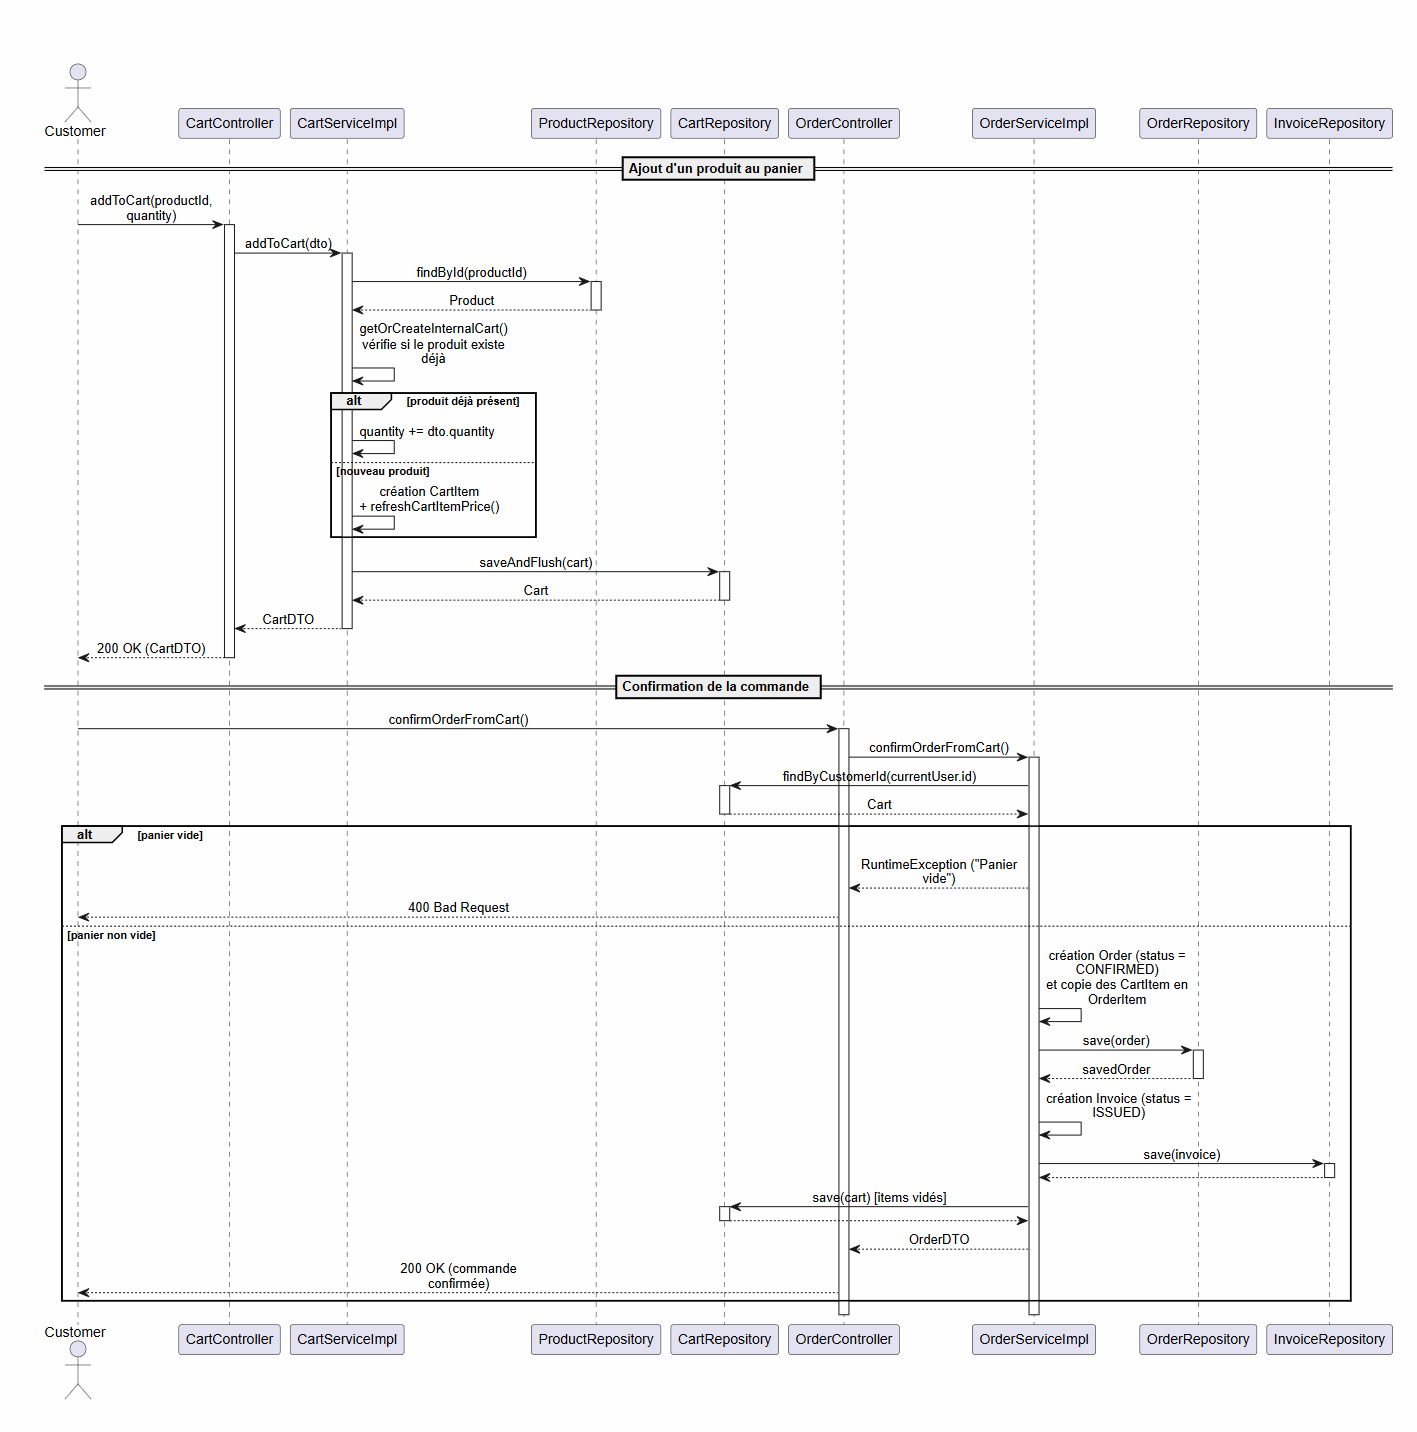
\includegraphics[width=1\textwidth]{images/uml/confirmCommande .png}
    \caption{Diagramme de séquence - Ajout au panier et confirmation d'une commande}
    \label{fig:sequence_confirmation_commande}
\end{figure}
\subsection{Diagramme de classes}

Le diagramme de classes ci-dessous (Figure~\ref{fig:diagramme-classes-sprint2}) représente la modélisation des entités du sprint 2, dédié à la \textbf{gestion des produits}. Il est organisé en trois grandes parties complémentaires :

\begin{itemize}
    \item \textbf{Le package Produit} : il modélise le catalogue de l'application autour de la classe abstraite \texttt{Product}, dont héritent deux types concrets, \texttt{Car} et \texttt{SparePart}, selon une stratégie d'héritage \texttt{SINGLE\_TABLE} avec discriminant. Chaque produit est rattaché à une \texttt{Category} et une \texttt{Brand}.

    \item \textbf{Le package Stock \& Fournisseur} : il gère l'approvisionnement. Chaque produit possède un \texttt{Stock} unique, dont l'évolution est tracée par des \texttt{StockMovement} (entrées/sorties). Les fournisseurs (\texttt{Supplier}) sont liés aux produits via \texttt{SupplierProduct}, qui centralise les conditions d'achat (prix, quantité minimale, fournisseur préféré). Les commandes fournisseurs (\texttt{PurchaseOrder}, \texttt{PurchaseOrderItem}) donnent lieu à une \texttt{PurchaseInvoice}, elle-même réglée via un ou plusieurs \texttt{SupplierPayment} découpés en \texttt{SupplierPaymentLine}.

    \item \textbf{Le package Commande, Panier \& Paiement} : il couvre le parcours client, depuis le \texttt{Cart} (panier) et ses \texttt{CartItem}, jusqu'à la validation d'une \texttt{Order} composée de \texttt{OrderItem}. Chaque commande génère une \texttt{Invoice} et est réglée par un \texttt{Payment}, lui-même décomposé en plusieurs \texttt{PaymentLine} pour permettre les paiements mixtes (ex. espèces + chèque).
\end{itemize}

La classe \texttt{PaymentMethod} est mutualisée entre les deux flux financiers (client et fournisseur), garantissant une gestion homogène des moyens de paiement (espèces, chèque, carte, virement, crédit) dans l'ensemble de l'application.

\begin{figure}[H]
    \centering
    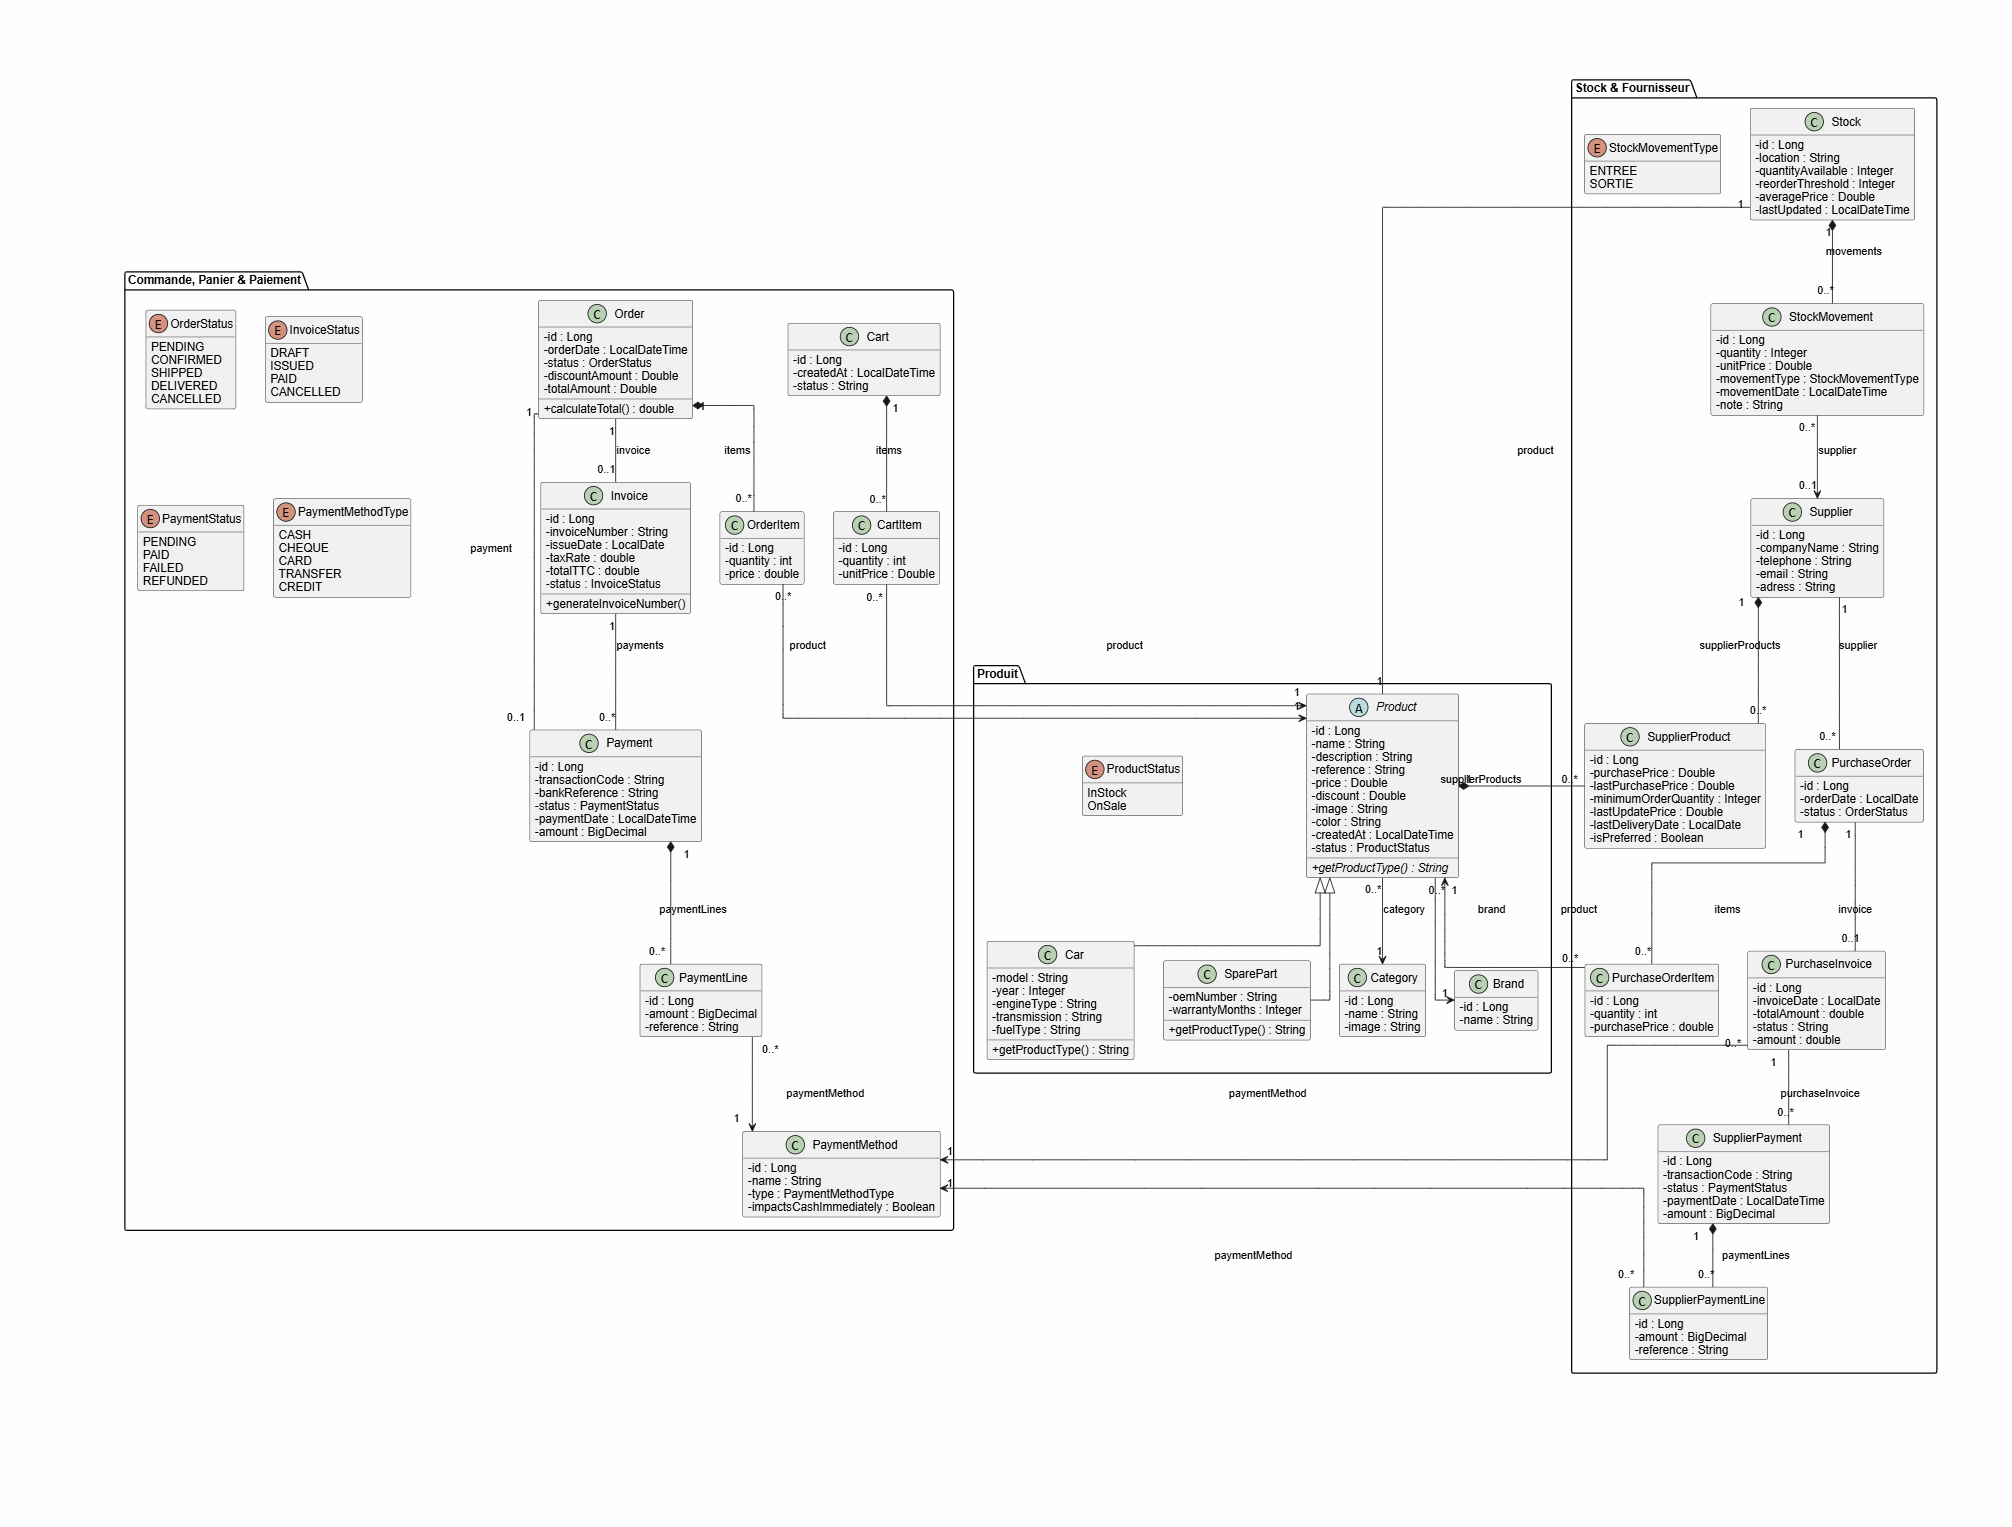
\includegraphics[width=\textwidth]{images/uml/diagDeClasseSprint2.png}
    \caption{Diagramme de classes du sprint 2 - Gestion des produits}
    \label{fig:diagramme-classes-sprint2}
\end{figure}
\section{Réalisation}

\subsection{Gestion des produits}

\subsubsection{Consultation et liste des produits}

\subsubsection{Recherche, filtrage et tri des produits}

\subsubsection{Ajout d'un produit}

\subsubsection{Modification d'un produit}

\subsubsection{Gestion des catégories}

\subsubsection{Gestion des marques}

\subsection{Gestion du stock}

\subsubsection{Consultation du stock}

\subsubsection{Réception d'une livraison}

\subsubsection{Ajustement des quantités}

\subsubsection{Gestion des mouvements de stock}

\subsubsection{Détection des produits en stock faible}

\subsection{Gestion des fournisseurs}

\subsubsection{Liste et recherche des fournisseurs}

\subsubsection{Ajout et modification d'un fournisseur}

\subsection{Gestion du panier et des commandes}

\subsubsection{Ajout des produits au panier}

\subsubsection{Gestion des quantités et suppression des articles}

\subsubsection{Gestion des demandes de maintenance dans le panier}

\subsubsection{Création et suivi des commandes}

\subsection{Gestion des factures et des paiements}

\subsubsection{Génération et consultation des factures}

\subsubsection{Gestion des méthodes de paiement}

\subsubsection{Traitement du paiement}

\subsubsection{Mise à jour du stock après paiement}

\subsubsection{Gestion de la caisse}

\section{Bilan du Sprint}